% -----------------------------------------------------------------------------
% Fundamentação Teórica
% -----------------------------------------------------------------------------

\chapter{Fundamentação Teórica}
\label{chap:fundamentacaoTeorica}

\section{Análise de dados em saúde}

Tomar decisões em saúde sempre precisam do suporte de um profissional especializado na temática a ser decidida. Uma série de técnicas são aplicadas por esse profissional para avaliação do contexto, uma vez que os dados puros não são suficientes pela multifatoriedade \cite{andrade_tomada_2008,resende2009}. Com o grande número de sistemas de auxílio em saúde, sejam de ordem regulatória ou ainda por iniciativas privadas, o volume de dados cresce exponencialmente, produzindo fenômeno de Big Data. Uma definição conhecida desse conceito aponta volume, variedade e velocidade como os três vetores relacionados à produção massiva de dados \cite{laney20013d}. Outras características foram adicionadas a essa primeira definição de Big Data, tais como veracidade \cite{schroeck2012analytics},  complexidade e desestruturação \cite{intel2012}, valor \cite{oracle2013}.

A multifatoriedade citada acima é um aspecto que se relaciona a complexidade dos dados em grande volumes, é cada vez mais difícil estabelecer uma relação de causa efeito para a tomada de decisão segura, sem auxílio ou sumarização desses dados em informações mais tangíveis e associadas. Ao mesmo tempo que é extremamente difícil de descrever um algoritmo suficiente que permita analisar todos os dados de contexto e relacioná-los de forma que possa ser utilizado como substituição ao conhecimento tácito de um profissional da saúde experiente \cite{faceli2011}.

O suporte de sistemas, métodos e pŕaticas que suportem tanto a assistência em saúde no tratamento de Big Data  ainda não é suficientemente consolidado. Faltam evidências de aplicações especialmente quantitativas que validem seu uso nesse campo do conhecimento. Além disso boa parte das tecnologias relacionadas em diversos estudos, utilizam tecnologias que demandam recursos específicos. Não obstante essa análise, estão focadas na avaliação de dados para otimização de recursos, suporte a decisões clínicas e redução de custo do cuidado \cite{nishita2018}.

Havendo ainda uma grande oportunidade de estudo para a área de processamento de dados que sumarizam informações e tornem mais fácil seu estudo, correlação e posteriormente associação com demais bancos, ou conjuntos de informações que é justamente o que esse trabalho se propõe, ainda que o volume de dados da base analisada neste trabalho e sua composição não qualifiquem como Big data, sob a perspectiva de LANEY. Pode ser utilizado de base para uma nova forma de utilização de recursos computacionais na análise de grandes massas de dados e a posteriori Big Data. 

\section{Alternativas open source}

A pesquisa sobre estratégias para a análise de dados retornou um grande número de artigos, sendo encontradas estratégias diversas descritas na literatura científica.  Para fins de apresentação dessas soluções neste trabalho, elas foram agrupadas conforme níveis de complexidade de implementação, sempre mantendo o custo como restrição primária e o contexto de aplicação em instituições com grande restrição orçamentária.
Diante disso, e tendo em vista o tamanho da base de dados de origem, durante o levantamento do projeto foram avaliadas soluções em duas categorias:

\begin{itemize}
    \item Computação em nuvem privada; e
    \item Orquestração de Containers.
\end{itemize}

Na primeira categoria, a utilização de ferramentas como OpenStack\textregistered e CloudStack\textregistered foram consideradas. No entanto, observa-se que nesse tipo de utilização existe um overhead substancial, tanto em termos de complexidade de configuração, quanto em termos de hardware necessário para operar de maneira eficiente. Essas alternativas requerem maior capacidade computacional, conforme suas configurações recomendadas \cite{cloudstack,openstack}. Além disso, as soluções de nuvem privada estendem muito o propósito de orquestração de cargas de trabalho, provendo todo o conceito de infraestrutura como serviço (Iaas). E, dependendo da implementação e dos componentes utilizados, elas provêm plataforma como serviço (PaaS), que são categorias de abstração do hardware, configurações e sistemas de suporte/apoio como Sistemas Operacionais (OS) para aplicação \cite{openstack,cloudstack,mell_nist_2011}. Logo, embora sejam alternativas populares, tornam o processo substancialmente mais complexo e, portanto, foram descartadas para essa avaliação tendo em vista o escopo deste trabalho.

Na segunda categoria, sistemas de orquestração de containers possuem um baixo overhead devido a arquitetura do container \ref{fig:container}, compartilhando parte do kernel space. Logo, não necessita de uma camada de virtualização do sistema operacional, presente em virtualizações completas e gerenciadas por hypervisors \ref{fig:vmscontainer}. Vale ressaltar que essa solução oferece ainda algumas possibilidades como, por exemplo,  o gerenciamento de capacidade dos nós do cluster para agendamento de tarefas. Dentre as plataformas disponíveis, o Kubernetes\textregistered é apontado como uma das principais soluções de orquestração de containers, tanto pela disponibilidade de features, quando pelos projetos em operação e pelo tamanho de sua comunidade \cite{truyen_comprehensive_2021}. O Kubernetes\textregistered tem o apoio de entidades como Cloud Native Computing Foundation (CNCF), que apoiam e supervisionam a plataforma de software -  definida como peça importante de software, sob o qual diversos programas de aplicativos menores podem ser projetados para serem executados \cite{collins2022}. Esse apoio tem como objetivo a expansão  das capacidades, endereçando problemas conhecidos e situações de uso, bem como estabelecendo padrões para tecnologias que pertencem ao ecossistema de orquestração de containers.

\begin{figure}[!h]
    \centering
    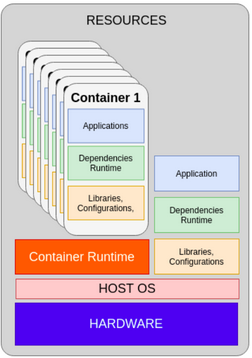
\includegraphics[width=0.3\textwidth]{04-figuras/containers.png}
    \caption{Estrutura do container (elaborada pelo autor)}
    \label{fig:container}
\end{figure}

\begin{figure}[!h]
    \centering
    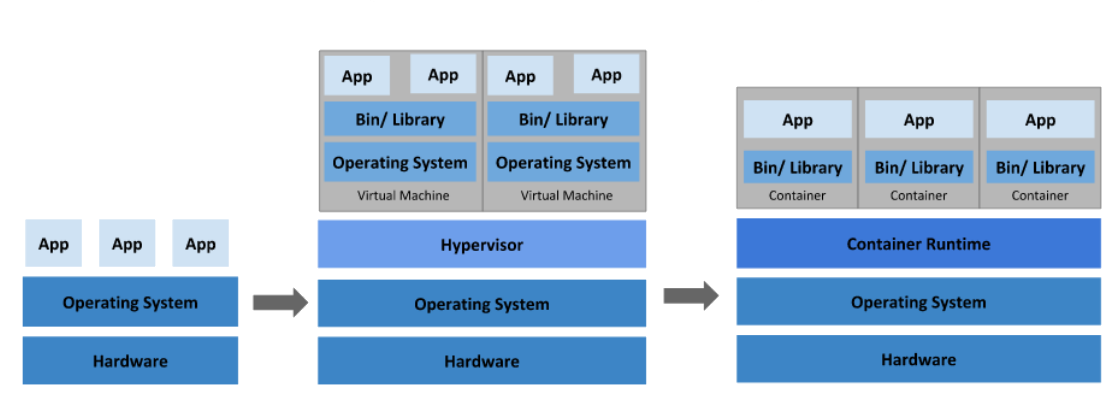
\includegraphics[width=0.8\textwidth]{04-figuras/vmsContainer.png}
    \caption{Eras de deployments e sua evolução por tecnologia base (Fonte: The Linux Foundation\textregistered, 2021)}
    \label{fig:vmscontainer}
\end{figure}

Soluções como Apache Mesos, Hashicorp Nomad, e Docker Swarm também foram avaliadas pelo estudo \cite{truyen_comprehensive_2021}, mas em todos os casos foram citadas diferenças significativas, especialmente no uso, sendo o Kubernetes\textregistered a melhor avaliada. 

\section{Cluster orquestrador de container}

Kubernetes\textregistered é a consolidação de quinze anos de trabalho da Google\textregistered com orquestração de cargas de trabalho, processamentos \emph{batch}, e um sistema interno de gerenciamento de cluster orientado a containers, o Borg \cite{verma_large-scale_2015}. 

As estruturas básicas do Kubernetes\textregistered são divididas em componentes com atribuições bem definidas \ref{fig:vmscontainer}. Os componentes que são essenciais a proposta deste trabalho são:
\begin{itemize}
    \item Kube-apiserver que concentra toda a api do kubernetes
    \item Kube-scheduler que avalia novos pods e em qual nó worker do cluster os mesmo serão alocados
    \item Kube-controller-manager que comporta os objetos de controle do kubernetes
    \item Kubelet responsável por repassar comando do control plane, para o worker e comunicar com container runtime
    \item Kube-proxy responsável por toda a estrutura de redes nativa do kubernetes e pods do cluster
    \item Pod menor unidade de deployment podendo conter um conjunto de containers que compõem uma solução.
\end{itemize}

\begin{figure}[!h]
    \centering
    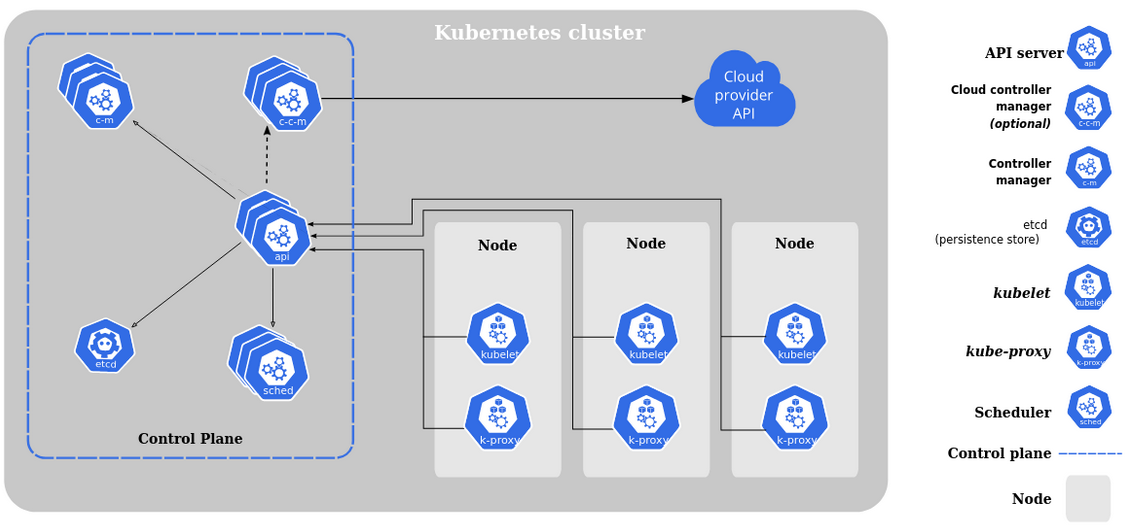
\includegraphics[width=0.8\textwidth]{04-figuras/kubeadm-node.png}
    \caption{Kubernetes arquitetura de componentes (Fonte: The Linux Foundation\textregistered, 2021)}
    \label{fig:kubenode}
\end{figure}



